\documentclass[11pt,a4paper]{article}
\usepackage[margin=18mm]{geometry}
\usepackage[T1]{fontenc}
\usepackage[utf8]{inputenc}
\usepackage{lmodern}
\usepackage{amsmath}
\usepackage{graphicx}
\usepackage{booktabs}
\usepackage{caption}
\usepackage{float}
\usepackage{enumitem}
\usepackage[hidelinks]{hyperref}
\graphicspath{{figures/}}
\captionsetup{font=small,labelfont=bf}
\setlist{nosep,leftmargin=*}
\setlength{\parskip}{3pt}
\setlength{\parindent}{0pt}

\begin{document}
\begin{center}
{\Large\textbf{Part 2: Transistor-Level ML Models}}\\[2pt]
ML-Driven PVT-Variation-Aware Leakage Estimation \quad$\cdot$\quad Member 2: Pranav Adarsh
\end{center}

\section*{Data and method}
Each of the four transistor cases (NMOS/PMOS, ON/OFF; 22\,nm MGK, ngspice, junction areas
$AD=AS=W\times2L_\mathrm{min}$) has 10,000 SPICE rows: 5,000 with $V_\mathrm{d}, V_\mathrm{s}$ uniform
in $[0,V_\mathrm{DD}]$ and 5,000 targeted at the voltages transistors see inside gates. The 12 inputs
($V_\mathrm{DD}$, temperature, $W$, terminal voltages, vth0, toxe, ndep, u0, xj) predict
$I_\mathrm{d}, I_\mathrm{g}, I_\mathrm{s}, I_\mathrm{b}$. Data is split 70/15/15 with a fixed seed (42).

Because currents span 15 decades, each model predicts $y=\log_{10}|I|$ and a LightGBM classifier
predicts the sign, so $I=\operatorname{sign}(I)\cdot10^{y}$. The inputs are extended with
physics-based features: voltage differences, $1/kT$, log process parameters and subthreshold
exponents such as $(V_\mathrm{gs}-|\mathrm{vth0}|)/kT$.

\section*{Models and selection}
The four families were chosen to span the main kinds of regression model, from a simple baseline
to a flexible neural network, so the comparison shows how much model complexity the leakage
problem needs:
\begin{itemize}
  \item \textbf{Polynomial ridge} (degree 2--3): the baseline. It is fast and interpretable and
        tests whether a smooth fixed functional form of the physics features is enough.
  \item \textbf{Random forest} (400 trees): a robust, widely used non-linear model that needs no
        feature scaling and little tuning, giving a reference for tree-based methods.
  \item \textbf{LightGBM} (boosted trees, early stopping): usually the most accurate model on
        tabular data such as SPICE sweeps, and fast to train.
  \item \textbf{MLP} (3$\times$64 tanh, L-BFGS): a smooth function approximator suited to the
        continuous, exponential device equations; one network predicts all four currents, so they
        share what it learns about the device.
\end{itemize}
For each case the model with the lowest validation score, mean over terminals of
$(\text{median}+\text{p95})/2$ relative error, was chosen.

\begin{table}[H]
\centering\small
\begin{tabular}{lcccc|cc}
\toprule
 & \multicolumn{4}{c|}{Validation median / p95 error (\%)} & \multicolumn{2}{c}{Test median / p95 (\%)} \\
Case & Poly ridge & Rand.\ forest & LightGBM & MLP & uniform & targeted \\
\midrule
NMOS ON  & 14.0 / 74 & 13.3 / 68 & 5.8 / 31 & \textbf{2.8 / 29} & 2.1 / 8  & 4.5 / 51 \\
NMOS OFF & 19.4 / 99 & 9.1 / 51  & 5.5 / 33 & \textbf{2.8 / 12} & 2.6 / 11 & 3.5 / 15 \\
PMOS ON  & 12.4 / 67 & 12.9 / 61 & \textbf{5.4 / 30} & 2.5 / 37 & 5.0 / 21 & 6.7 / 40 \\
PMOS OFF & 21.0 / 94 & 9.9 / 52  & 5.5 / 31 & \textbf{2.9 / 13} & 2.6 / 13 & 3.3 / 14 \\
\bottomrule
\end{tabular}
\caption{Model comparison (mean of four terminals). Bold: chosen model; test columns are for the
chosen model.}
\label{tab:results}
\end{table}

\section*{Results}
The MLP had the lowest median error in every case and was chosen for NMOS ON, NMOS OFF and PMOS OFF.
For PMOS ON, LightGBM won on the selection score (17.6 vs 19.7) through its better p95, although
the MLP's median is lower; the rule's choice was kept (using the MLP changes gate accuracy by under
0.1 point). On the test sets the chosen models reach 2.1--2.6\% median error on typical points
(5.0\% for PMOS ON), with $R^2 \ge 0.98$ on $\log_{10}|I|$ and the correct sign in 98--100\% of rows
(Table~\ref{tab:results}). The largest errors are the OFF body current (junction leakage) and the
ON-device $I_\mathrm{d}, I_\mathrm{s}$ at $V_\mathrm{ds}\approx0$, which the gate formula does not use.

Used in Parts 3 and 4, the models give \textbf{1.33\% median error (98.2\% mean accuracy)} over
3,600 gate simulations and \textbf{1.14\% median (98.6\% mean accuracy)} over 102,400 simulations of
the 9-input parity checker. The learning curve shows the OFF and PMOS ON models still improving at
7k training rows, so more targeted data or an MLP ensemble could close the gap to 99\%.

\begin{figure}[H]
\centering
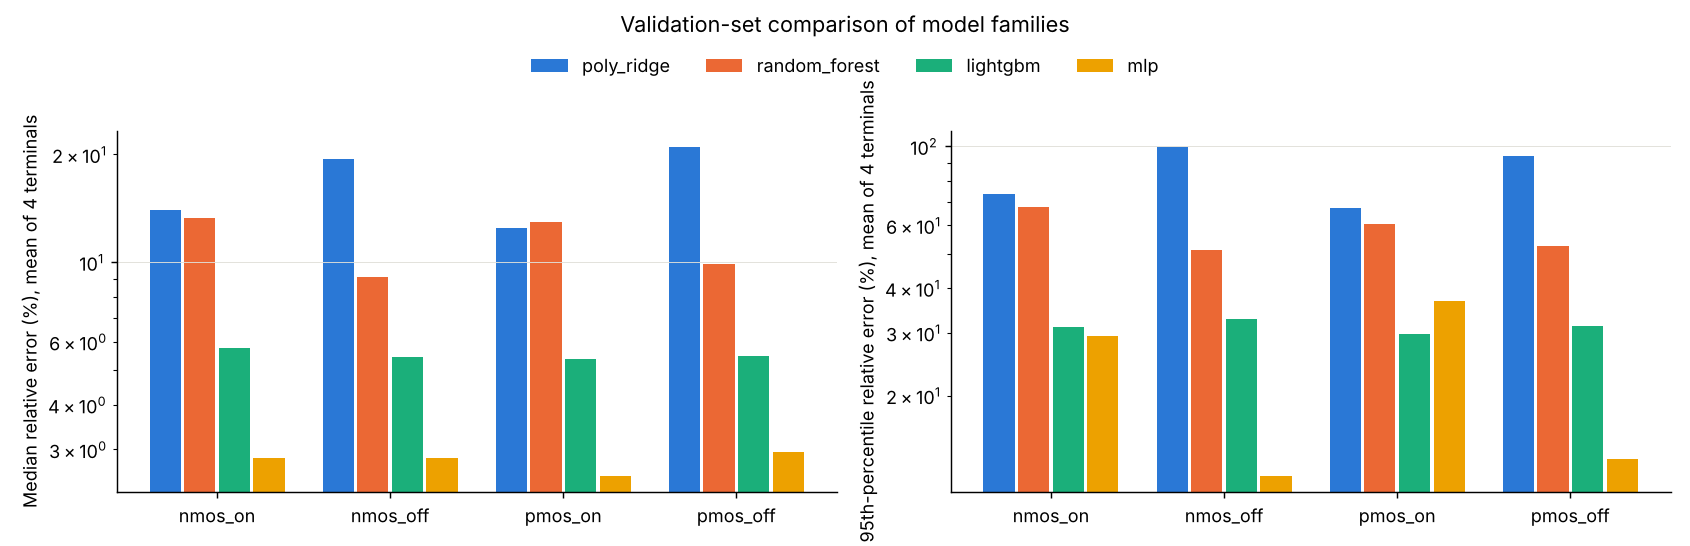
\includegraphics[width=\linewidth]{family_comparison.png}
\caption{Validation error of the four model families per case: median (left) and p95 (right).}
\end{figure}

\begin{figure}[H]
\centering
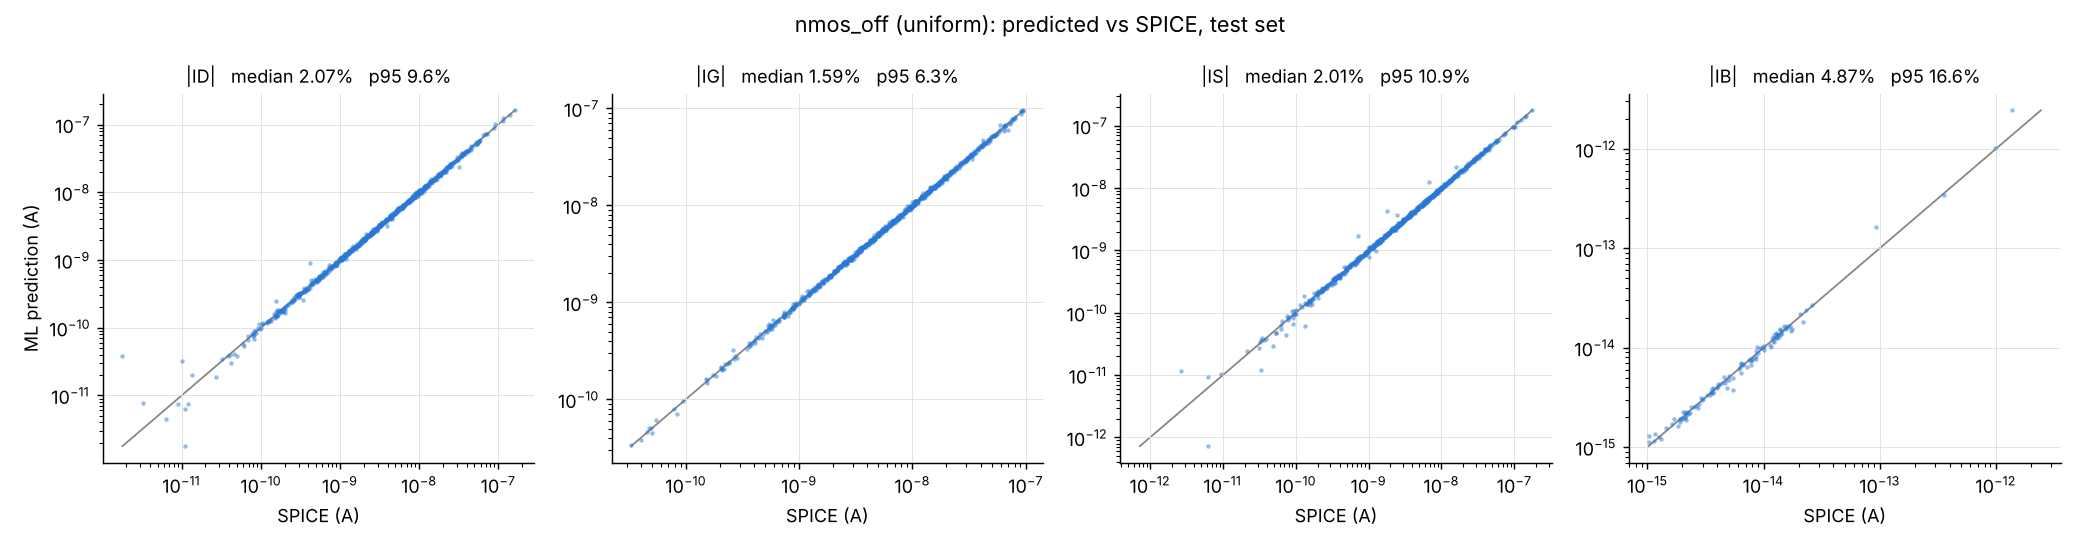
\includegraphics[width=\linewidth]{parity_nmos_off.png}
\caption{Predicted vs SPICE currents, NMOS OFF, uniform test set.}
\end{figure}

\begin{figure}[H]
\centering
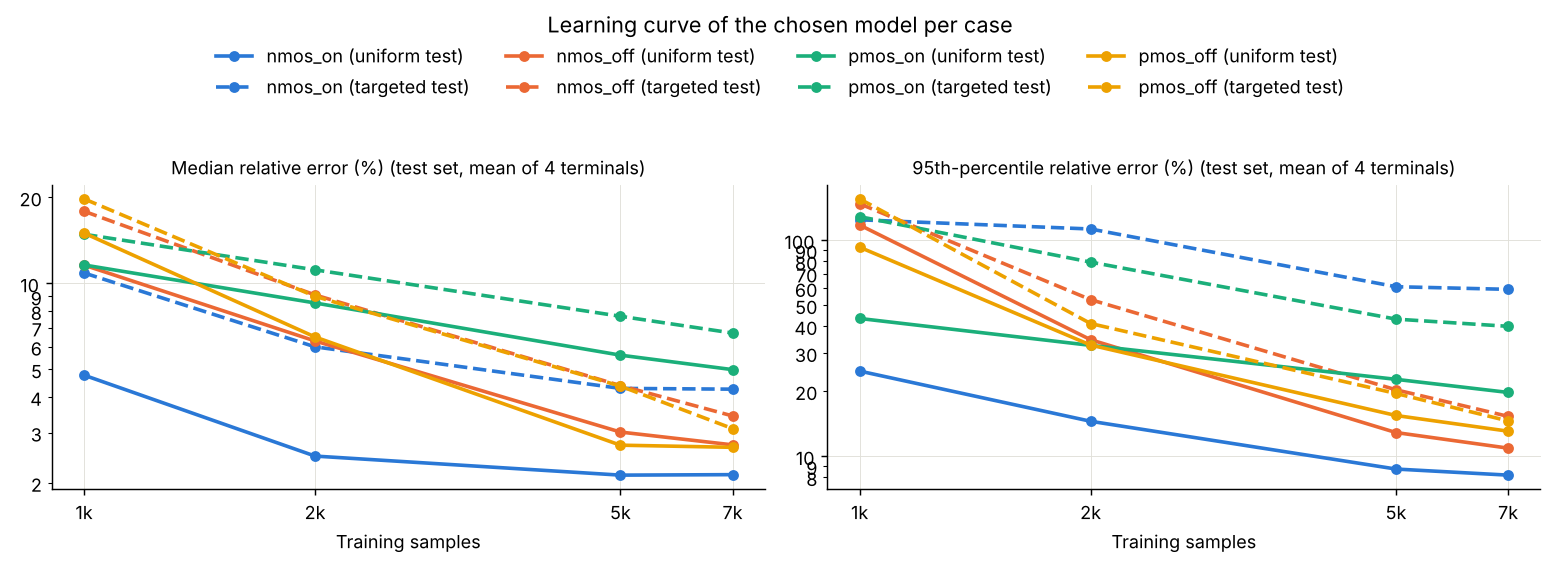
\includegraphics[width=\linewidth]{learning_curve.png}
\caption{Learning curve of the chosen model per case (solid: uniform test; dashed: targeted test).}
\end{figure}

\begin{figure}[H]
\centering
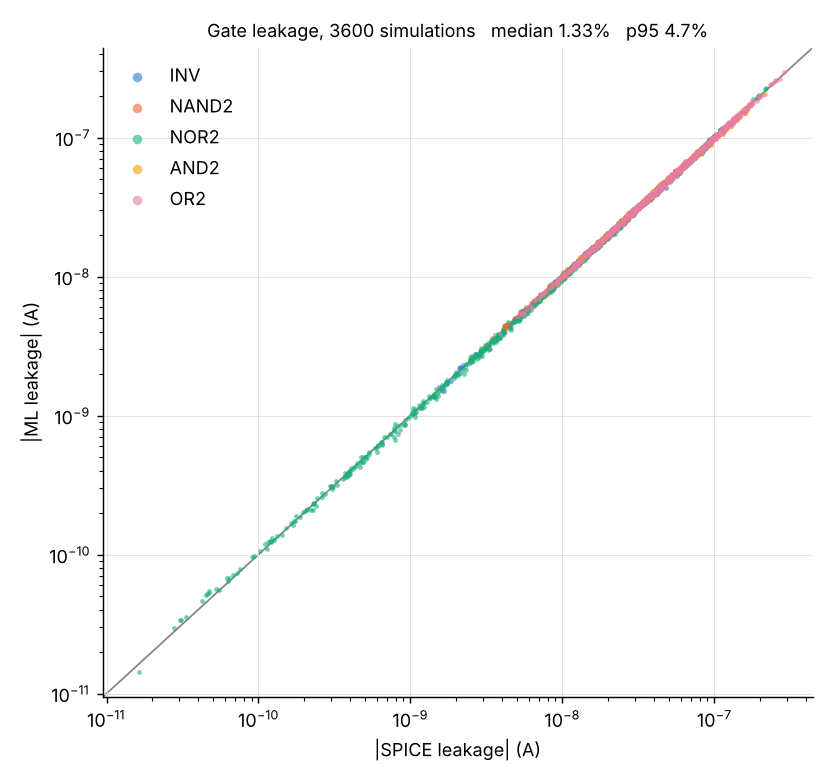
\includegraphics[width=0.55\linewidth]{gate_parity.png}
\caption{Gate leakage, ML vs SPICE, over all 3,600 gate simulations.}
\end{figure}

\end{document}
